\section{An\'alise dos resultados}
\label{sec:resultados}

% Passa-se ao tratamento dos dados por intermédio dos testes estatísticos, os quais dependem das hipóteses a serem testadas. Nesse tópico, é exigido que sejam aplicados testes de hipóteses paramétricos e/ou não paramétricos. Testes de duas amostras são exigidos quando comparando abordagens




%\begin{figure}[t]
%    \centering
%    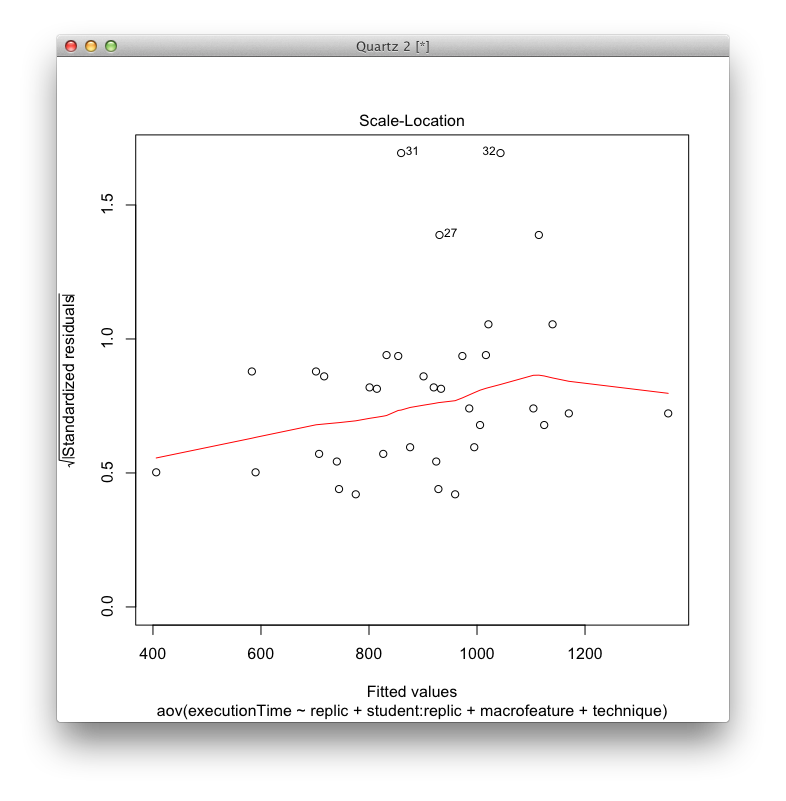
\includegraphics[width=0.6\textwidth]{images/grafico2.png}
%    \caption{}
%    \label{fig:grafico2}
%\end{figure}

%\begin{figure}[t]
%    \centering
%    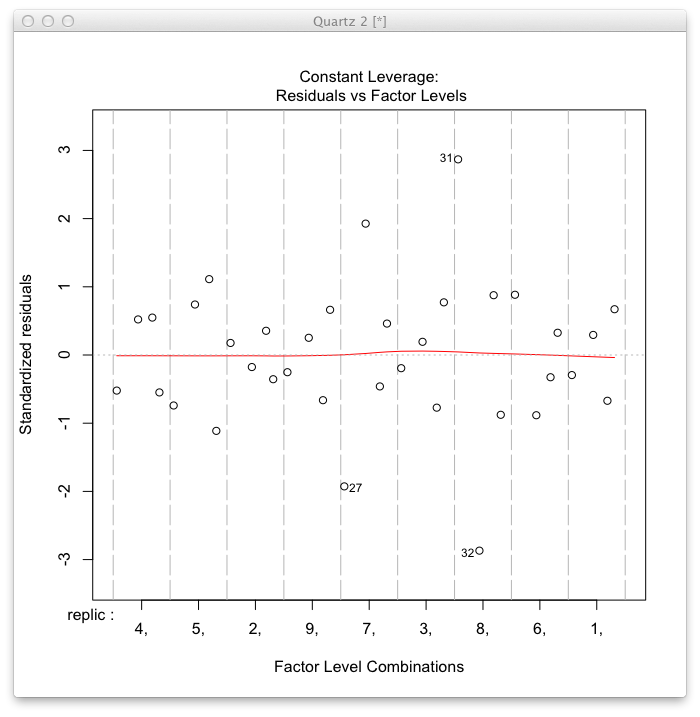
\includegraphics[width=0.6\textwidth]{images/grafico3.png}
%    \caption{}
%    \label{fig:grafico3}
%\end{figure}

%\begin{figure}[t]
%    \centering
%    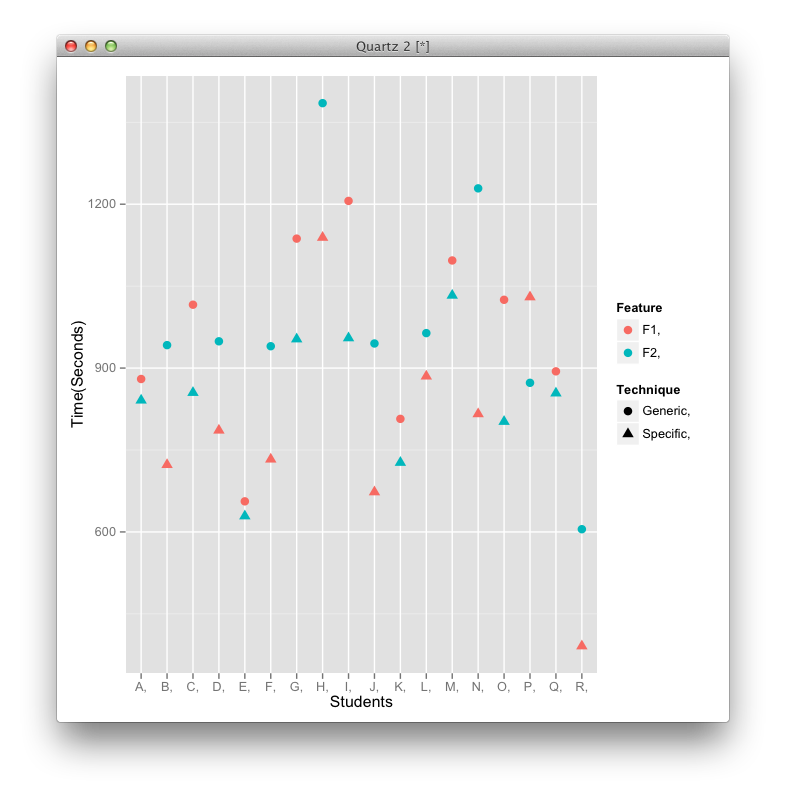
\includegraphics[width=0.6\textwidth]{images/dotplot.png}
%    \caption{}
%    \label{fig:dotplot}
%\end{figure}